%----------------------------------------------------------------------------------------
%       ANEXO C: CERTIFICADOS Y RECONOCIMIENTOS
%----------------------------------------------------------------------------------------
\chapter{Certificados y Reconocimientos}
\label{anexo:certificados}

Este anexo presenta los certificados, reconocimientos y constancias de participación obtenidos durante el desarrollo de esta investigación. Estos documentos dan testimonio de la difusión de los resultados en congresos, jornadas académicas y eventos científicos organizados por instituciones nacionales e internacionales, así como de actividades de divulgación relacionadas con visión por computadora y aprendizaje profundo.

\section{Reconocimiento - Encuentro NOVA}

\textbf{Evento:} Encuentro de Jóvenes Investigadores NOVA (Evento INSIGNIA NOVA)

\textbf{Fecha:} 12 y 13 de noviembre de 2025

\textbf{Lugar:} Auditorio de la Facultad de Ciencias de la Electrónica, Benemérita Universidad Autónoma de Puebla

\textbf{Institución organizadora:} Rama Estudiantil IEEE BUAP

\textbf{Tipo de participación:} Presentación de poster científico

\textbf{Título del trabajo presentado:} ``Normalización y alineación automática de la forma de la región pulmonar integrada con selección de características discriminantes para detección de neumonía y COVID-19''

\textbf{Descripción:} Este reconocimiento se otorga por la presentación de un poster científico en el Encuentro NOVA, donde se expuso la metodología de normalización geométrica mediante landmarks y warping piecewise affine para la detección de neumonía y COVID-19. Este trabajo está directamente relacionado con la investigación central de esta tesis.

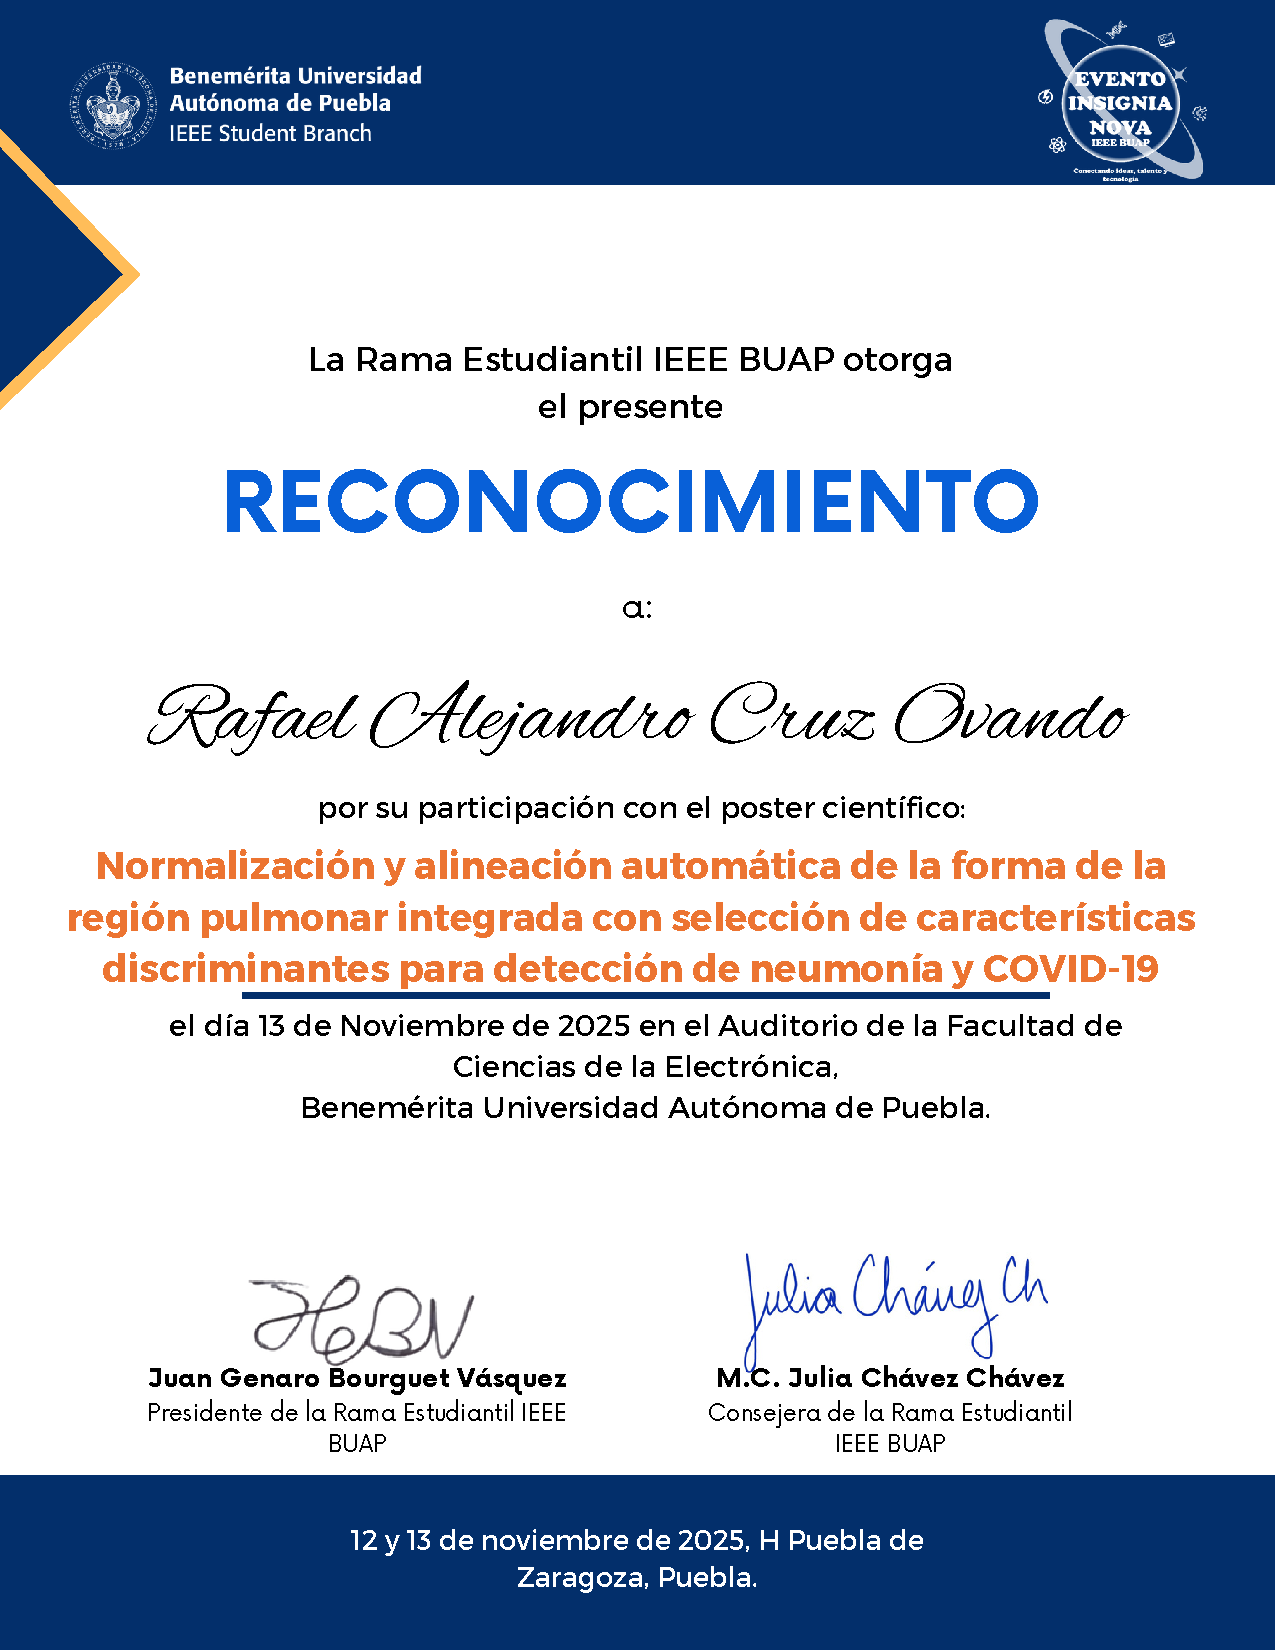
\includepdf[pages=-,pagecommand={\thispagestyle{plain}}]{anexos/reconocimiento_nova.pdf}

\section{Reconocimiento - IEEE DAY}

\textbf{Evento:} IEEE DAY

\textbf{Fecha:} 15 de octubre de 2025

\textbf{Institución organizadora:} IEEE Capítulo Estudiantil BUAP

\textbf{Tipo de participación:} Presentación técnica

\textbf{Título de la presentación:} ``Introducción a Redes Neuronales''

\textbf{Descripción:} Este certificado se otorga por la presentación técnica sobre fundamentos de redes neuronales en el evento IEEE DAY, organizado por la Rama Estudiantil IEEE de la Facultad de Ciencias de la Electrónica, BUAP. La presentación abordó conceptos fundamentales de redes neuronales, tema relacionado con las arquitecturas CNN utilizadas en el clasificador de esta tesis.

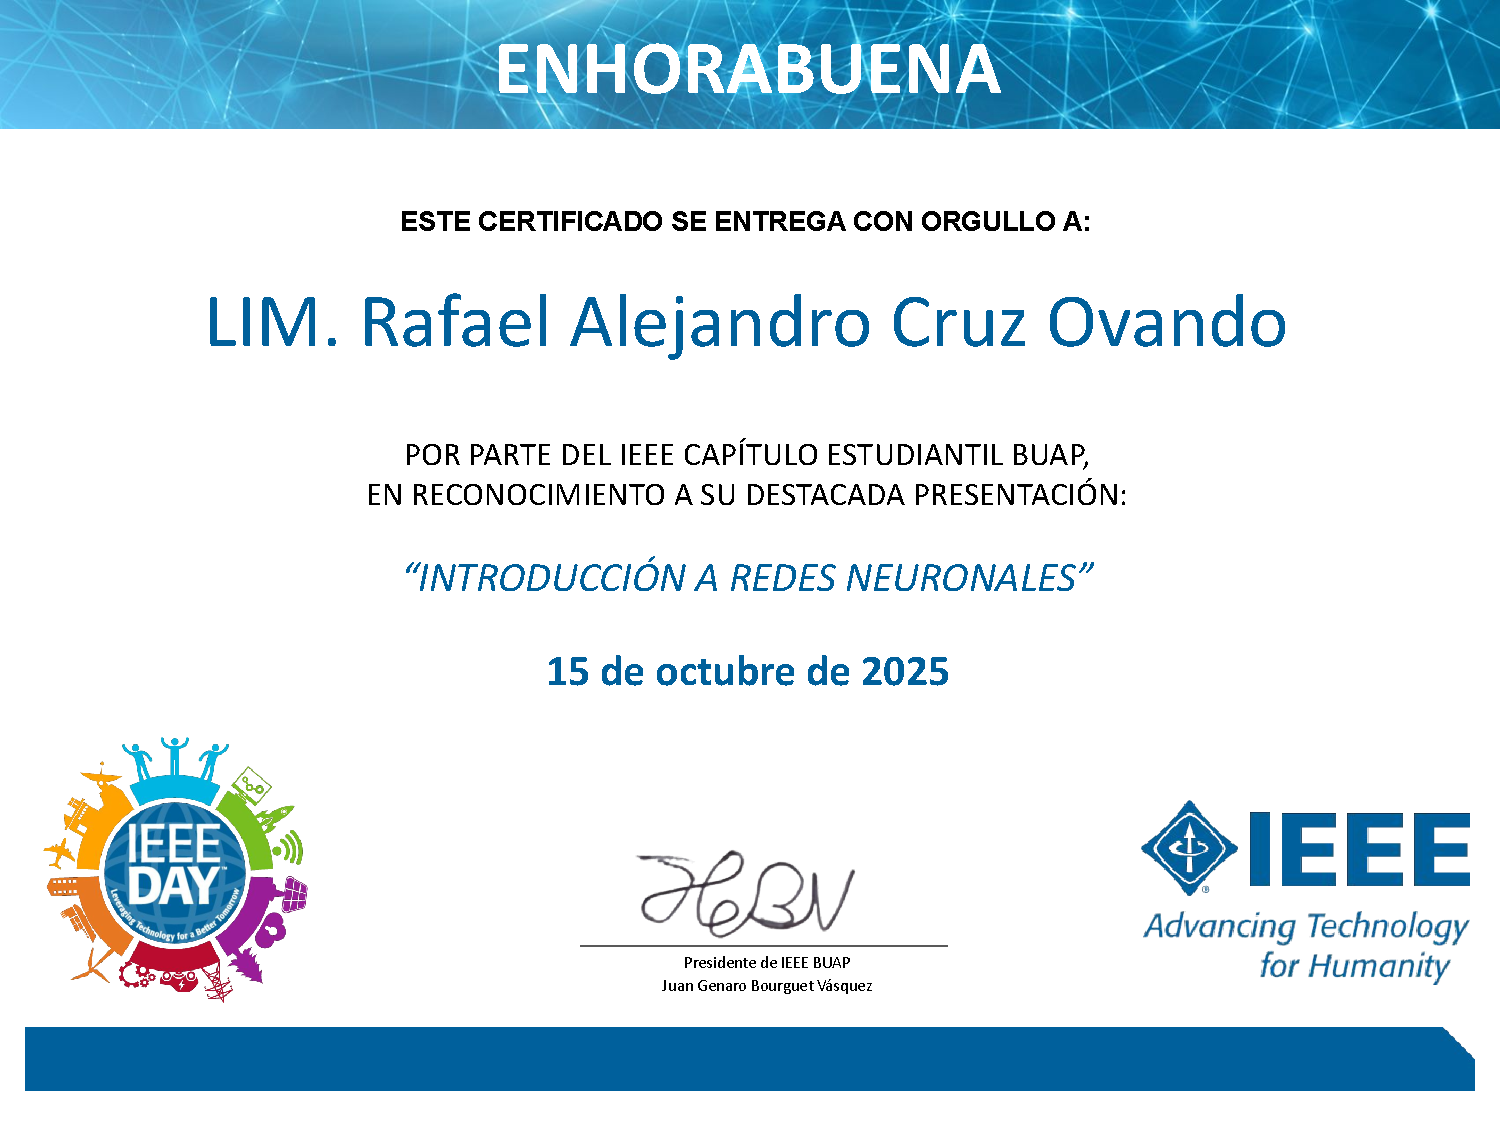
\includepdf[pages=-,pagecommand={\thispagestyle{plain}}]{anexos/reconocimiento_ieee_day.pdf}

\section{Constancia de Participación - RVP-AI ROC\&C 2025 y Congreso de Estudiantes IEEE}

\textbf{Evento principal:} RVP-AI ROC\&C 2025)

\textbf{Evento asociado:} Congreso de Estudiantes IEEE (28 y 29 de julio de 2025)

\textbf{Fecha:} 27 al 31 de julio de 2025

\textbf{Lugar:} Palacio Mundo Imperial, Riviera Diamante, Acapulco, Guerrero

\textbf{Institución organizadora:} IEEE Sección México

\textbf{Firmante:} Dr. Ricardo Mota Palomino (Presidente IEEE Sección México)

\textbf{Descripción:} Esta constancia acredita la participación en la Reunión de Verano de Potencia, Aplicaciones Industriales, Robótica y Organización de Comités (RVP-AI ROC\&C 2025), así como en el Congreso de Estudiantes IEEE, eventos organizados por la Sección México del IEEE. Estos eventos nacionales reúnen a estudiantes, académicos e investigadores para la difusión de trabajos en áreas de ingeniería eléctrica, electrónica, computación y disciplinas afines.

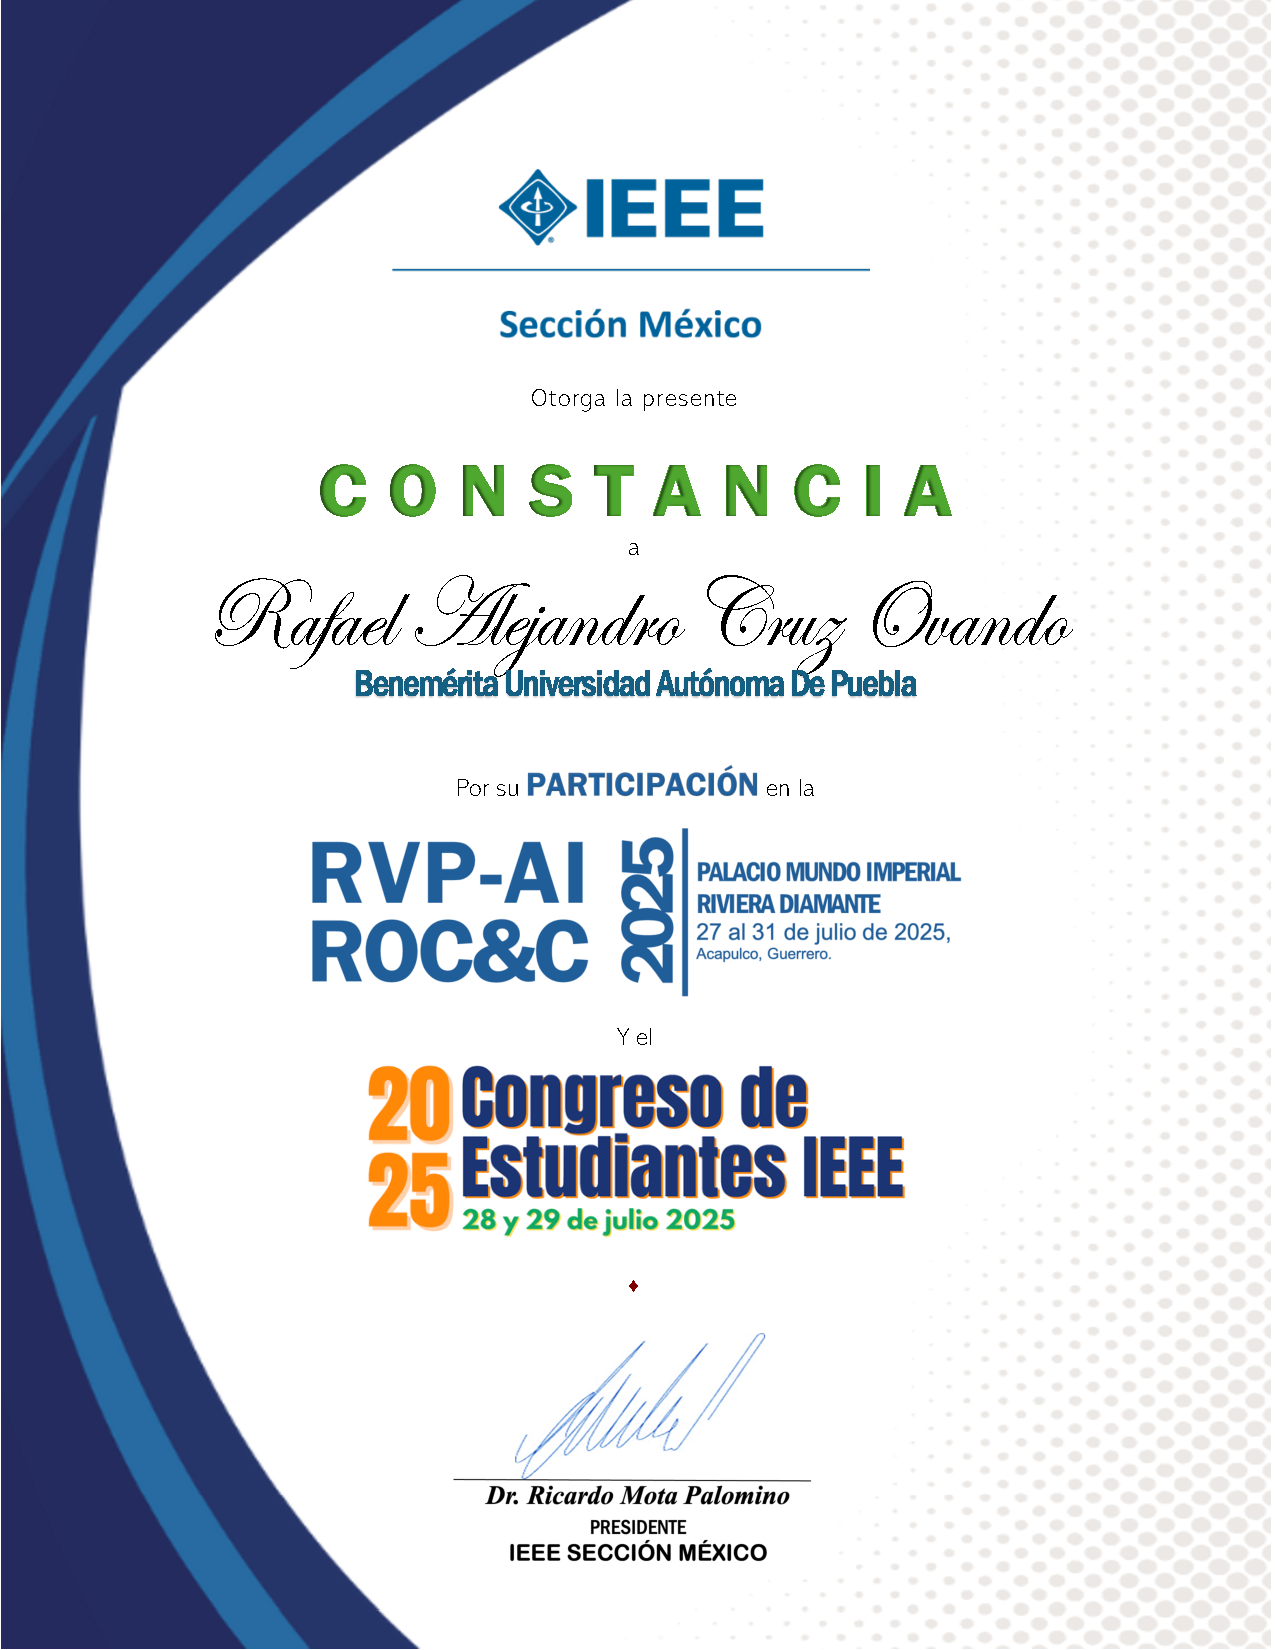
\includepdf[pages=-,pagecommand={\thispagestyle{plain}}]{anexos/constancia_participacion_rafael.pdf}

\section{Reconocimiento - Ponente en Taller de Visión por Computadora}

\textbf{Evento:} Taller ``Visión por Computadora''

\textbf{Fecha:} 17 de septiembre de 2025

\textbf{Lugar:} Facultad de Ciencias de la Electrónica, Benemérita Universidad Autónoma de Puebla

\textbf{Institución organizadora:} Sociedad de Robótica y Automatización (RAS) - IEEE BUAP

\textbf{Tipo de participación:} Ponente del taller

\textbf{Firmante:} Eder Yubaí Hernández Marcelino (Presidente RAS IEEE BUAP)

\textbf{Descripción:} Este reconocimiento se otorga por la participación como ponente en el taller de ``Visión por Computadora'', organizado por la Sociedad de Robótica y Automatización (RAS) del IEEE BUAP. El taller abordó temas de entrenamiento y prueba de redes neuronales convolucionales.

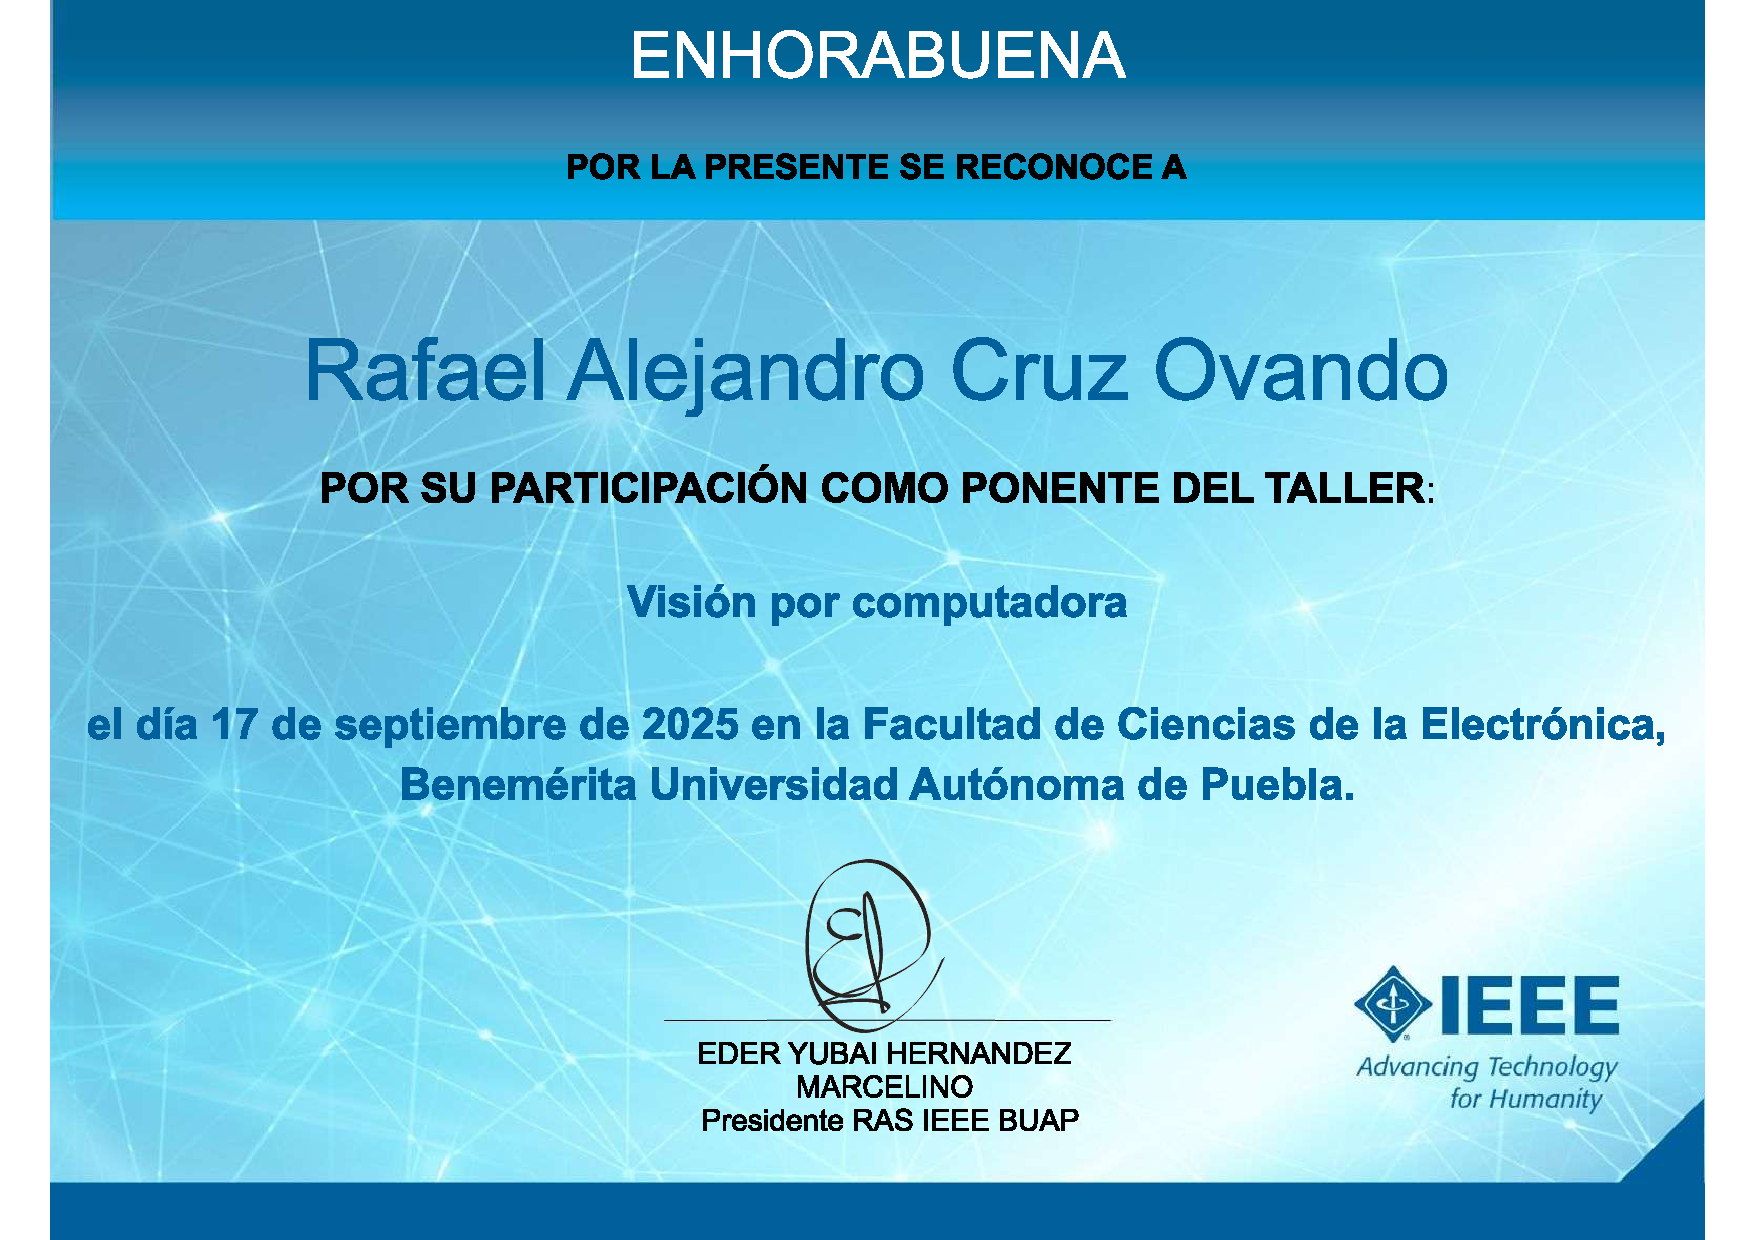
\includepdf[pages=-,pagecommand={\thispagestyle{plain}}]{anexos/reconocimiento_ras_day.pdf}
